% Credits are indicated where needed. The general idea is based on a template by Vel (vel@LaTeXTemplates.com) and Frits Wenneker.

\documentclass[11pt, a4paper]{article} % General settings in the beginning (defines the document class of your paper)
% 11pt = is the font size
% A4 is the paper size
% “article” is your document class

%----------------------------------------------------------------------------------------
%	Packages
%----------------------------------------------------------------------------------------

% Necessary
\usepackage[german,english]{babel} % English and German language 
\usepackage{booktabs} % Horizontal rules in tables 
% For generating tables, use “LaTeX” online generator (https://www.tablesgenerator.com)
\usepackage{comment} % Necessary to comment several paragraphs at once
\usepackage[utf8]{inputenc} % Required for international characters
\usepackage[T1]{fontenc} % Required for output font encoding for international characters

% Might be helpful
\usepackage{amsmath,amsfonts,amsthm} % Math packages which might be useful for equations
\usepackage{tikz} % For tikz figures (to draw arrow diagrams, see a guide how to use them)
\usepackage{tikz-cd}
\usetikzlibrary{positioning,arrows} % Adding libraries for arrows
\usetikzlibrary{decorations.pathreplacing} % Adding libraries for decorations and paths
\usepackage{tikzsymbols} % For amazing symbols ;) https://mirror.hmc.edu/ctan/graphics/pgf/contrib/tikzsymbols/tikzsymbols.pdf 
\usepackage{blindtext} % To add some blind text in your paper

% Images
\usepackage{graphicx}
\graphicspath{ {images/} }
\usepackage[utf8x]{inputenc}  % unicode
\usepackage{wrapfig}
\usepackage{lipsum}  % generates filler text

%---------------------------------------------------------------------------------
% Additional settings
%---------------------------------------------------------------------------------

%---------------------------------------------------------------------------------
% Define your margins
\usepackage{geometry} % Necessary package for defining margins

\geometry{
	top=2cm, % Defines top margin
	bottom=2cm, % Defines bottom margin
	left=2.2cm, % Defines left margin
	right=2.2cm, % Defines right margin
% 	includehead, % Includes space for a header
	%includefoot, % Includes space for a footer
	%showframe, % Uncomment if you want to show how it looks on the page 
}

\setlength{\parindent}{15pt} % Adjust to set you indent globally 

%---------------------------------------------------------------------------------
% Define your spacing
\usepackage{setspace} % Required for spacing
% Two options:
\linespread{1.5}
%\onehalfspacing % one-half-spacing linespread

%----------------------------------------------------------------------------------------
% Define your fonts
\usepackage[T1]{fontenc} % Output font encoding for international characters
\usepackage[utf8]{inputenc} % Required for inputting international characters

\usepackage{XCharter} % Use the XCharter font


%---------------------------------------------------------------------------------
% Define your headers and footers

\usepackage{fancyhdr} % Package is needed to define header and footer
\pagestyle{fancy} % Allows you to customize the headers and footers


%\renewcommand{\sectionmark}[1]{\markboth{#1}{}} % Removes the section number from the header when \leftmark is used

% Headers
\lhead{} % Define left header
\chead{\textit{}} % Define center header - e.g. add your paper title
\rhead{} % Define right header

% Footers
\lfoot{} % Define left footer
\cfoot{\footnotesize \thepage} % Define center footer
\rfoot{ } % Define right footer

%---------------------------------------------------------------------------------
%	Add information on bibliography
\usepackage{natbib} % Use natbib for citing
\usepackage{har2nat} % Allows to use harvard package with natbib https://mirror.reismil.ch/CTAN/macros/latex/contrib/har2nat/har2nat.pdf

% For citing with natbib, you may want to use this reference sheet: 
% http://merkel.texture.rocks/Latex/natbib.php

%---------------------------------------------------------------------------------
% Add field for signature (Reference: https://tex.stackexchange.com/questions/35942/how-to-create-a-signature-date-page)
\newcommand{\signature}[2][5cm]{%
  \begin{tabular}{@{}p{#1}@{}}
    #2 \\[2\normalbaselineskip] \hrule \\[0pt]
    {\small \textit{Signature}} \\[2\normalbaselineskip] \hrule \\[0pt]
    {\small \textit{Place, Date}}
  \end{tabular}
}
%---------------------------------------------------------------------------------
%	General information
%---------------------------------------------------------------------------------
\title{CS 4641 Project 1: Supervised Learning} % Adds your title
\author{
Sarah Chen % Add your first and last name
    %\thanks{} % Adds a footnote to your title
    %\institution{YOUR INSTITUTION} % Adds your institution
  }

\date{\small February 10, 2019} % Adds the current date to your “cover” page; leave empty if you do not want to add a date
% \lhead{CS 4641}
% \chead{Sarah Chen}
% \rhead{February 10, 2019}

%---------------------------------------------------------------------------------
%	Define what’s in your document
%---------------------------------------------------------------------------------

\begin{document}


% If you want a cover page, uncomment "\input{coverpage.tex}" and uncomment "\begin{comment}" and "\end{comment}" to comment the following lines
%\input{coverpage.tex}

%\begin{comment}
\maketitle % Print your title, author name and date; comment if you want a cover page 

\begin{center} % Center text
    % Word count: XXXX
% How to check words in a LaTeX document: https://www.overleaf.com/help/85-is-there-a-way-to-run-a-word-count-that-doesnt-include-latex-commands
\end{center}
%\end{comment}

%----------------------------------------------------------------------------------------
% Introduction
%----------------------------------------------------------------------------------------
\setcounter{page}{1} % Sets counter of page to 1

\section{Selected Classification Problems} % Add a section title
\subsection{Sentiment Analysis} % Add a subsection
Inherently, sentiment analysis is the process of computationally identifying and categorizing opinions or attitudes expressed in various strings of text. Sentiment analysis is interesting in many regards: in a world characterized by a rapid expansion of both technological power and freedom of speech, understanding the arguments and emotion behind scripts of text is more important than ever. Practical applications include understanding general political opinions, especially before elections, and determining customer satisfaction with commercial products, which is essential when conducting market research or gathering user experience. With the growth of social media users comes a growth in expressed points of view, and discovering these beliefs is vital to the success of businesses, politicians, and even the stock market.
\newline\newline 
For this project, I focused on predicting whether a string or passage was positive or negative, thereby branding it as a binary classification problem. Transcripts were taken from Twitter tweets and Yelp, IMDb, and Amazon reviews. My overall dataset consisted of a total of 24734 strings, each followed by a label: 0 if it carried a negative nuance, and 1 if it carried a positive nuance. The strings were divided into training and test sets using a 70/30 ratio. As the algorithms were running extremely slowly on my original set of 1.6 million tweets, I compressed its size down to 5000 arbitrarily chosen entries. It's important to note that this may affect the accuracy and error of my results as the tweets consist of a far wider range of words than the three sets of reviews, and diminishing the size of the collection of tweets means weakening the associations between some words (that may not appear in the reviews) and their nuances as well. 
% Moreover, the presence of outliers may be heightened, further complicating the algorithms' ability to learn the correct associations.
\subsection{Phishing Websites} % Add another subsection
If you are in anyway affiliated with Georgia Tech, surely, you must be familiar with the institute's infamous phishing emails, designed to help students, faculty, and staff learn how to identify phishing threats in an email. Predicting phishing seems to be a difficult problem due to the vagueness in identifying what attributes are associated with such emails. My dataset consists of 11000 entries of 31 attributes thought to be correlated with phishing, including URL length, presence of the ``@'' symbol, presence of a subdomain, and domain registration length. Each attribute has value 0 (missing) or 1 (present). Entries were partitioned into training and test sets using a 80/20 ratio.
% Citing in \LaTeX is easy. You could easier cite with the text flow like this ``Referring to \citet{collier2004greed} ...''  or at the end of the sentence \cite{collier2004greed}. You can also cite pages like this \citep[55]{collier2004greed}. If you want to add an additional note, you might want to do it this way \citep[cp.][22]{collier2004greed} or like this \citep[cp.][]{collier2004greed}.\\
% \blindtext % Adds some blintext to your text

%----------------------------------------------------------------------------------------
% Literature review
%----------------------------------------------------------------------------------------

\section{Sentiment Analysis}

\subsection{Algorithms} A bag-of-words model was used to aid these algorithms. An optimal bag size was determined for each by running the algorithm on various bag sizes while holding other variables constant. Afterwards, I observed the errors produced at each bag size, and used the size that generated the least error to run the algorithm as a function of training size.

\subsubsection{$K$-Nearest Neighbors}
In implementing the $k$-nearest neighbors method of classification, I found the optimal bag size to be 2500. An optimal value of $k$ was determined in a similar fashion by holding the bag size constant at 2500 items and examining the error produced by iterating over values of $k$ such that $3\leq k< 8$.
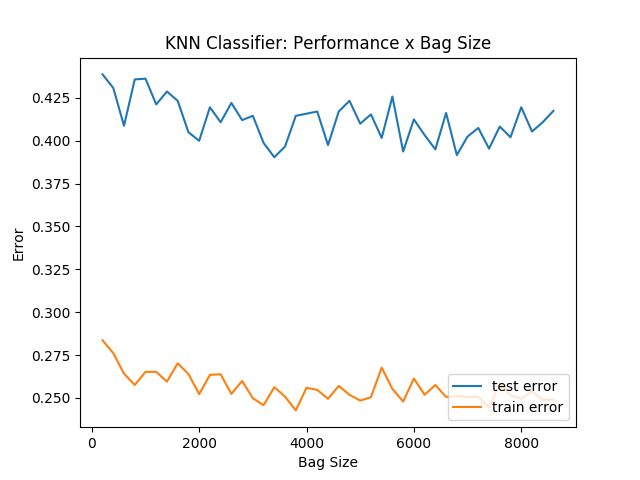
\includegraphics[scale=0.525]{kNN_BS.png}
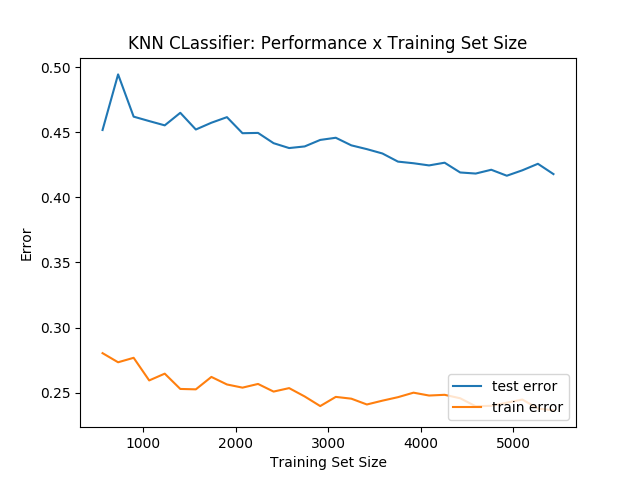
\includegraphics[scale=0.525]{kNN_TSS4.png}
\begin{wrapfigure}{L}{0.5\textwidth}
\centering
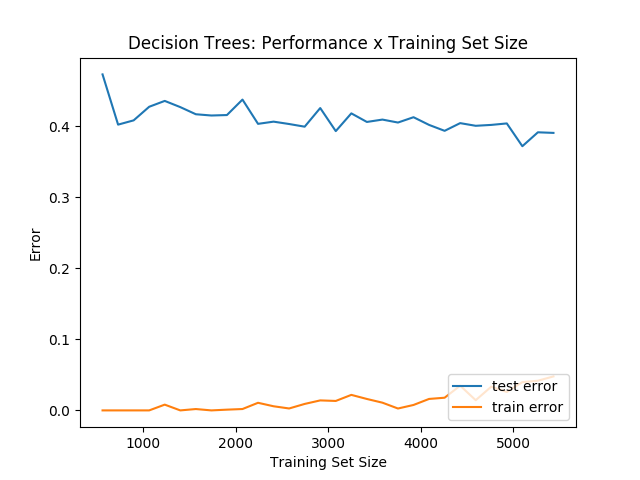
\includegraphics[scale=0.525]{DTTSS.png}
\end{wrapfigure}
It appears that $k=4$ produced the lowest error rate, albeit only by a small margin, so a bag size of 2500 and $k$ value of 4 were used to run the algorithm as a function of training size.
% \begin{center}
%     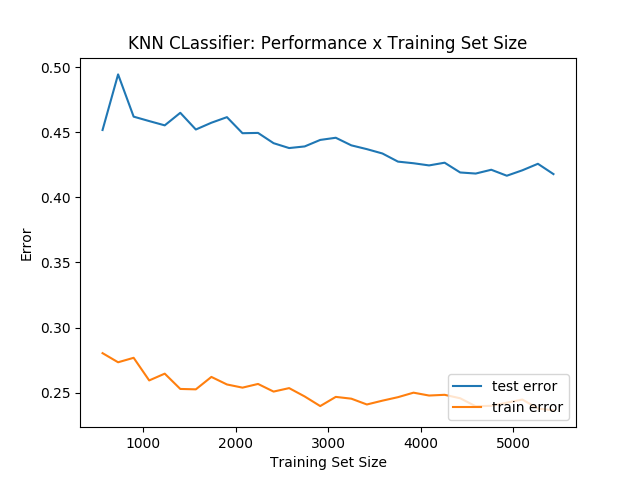
\includegraphics[scale=0.525]{kNN_TSS4.png}
% \end{center}
The results indicate that the error dropped from 0.50 (as good as randomly guessing) to approximately 0.42. The high error rate could be attributed to the fact that neutral words, including articles such as ``the'' and ``a'', are still classified as either positive or negative, therefore clouding the true sentiment value. For instance, if in a given iteration, ``the'' is attributed positively, and a negative sentence contains many appearances of ``the'', $k$-nearest neighbors would classify the sentence positively. This could be remedied by preprocessing the data to ignore neutral words using some sort of information theory analysis, perhaps by using pointwise mutual information. However, because $k$-nearest neighbors is a supervised learning algorithm, overall, the error trends downwards.

\subsubsection{Decision Trees}
The optimal bag size used in my decision tree implementation turned out to also be of size 2500. Pruning was accomplished through the limitation of the depth of the tree, or the maximum length of a path from the tree's root to one of the tree's leaves. Implementing the algorithm on trees with their depths limited to values between 2 and 50, I found that pruning with $\texttt{max depth}$=10 minimized the error. 
\newline\newline
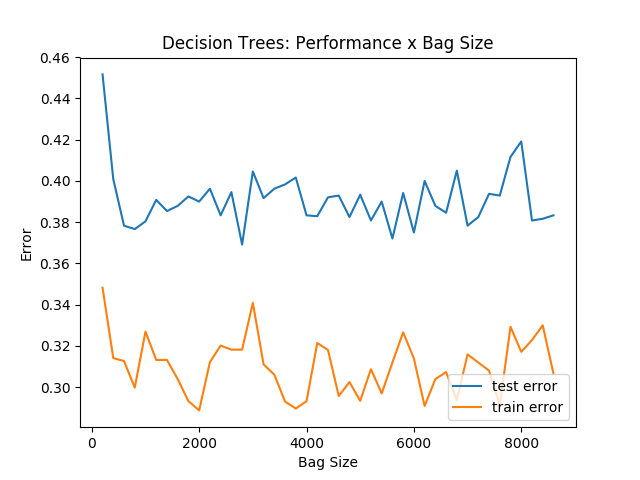
\includegraphics[scale=0.525]{DTBS2.png}
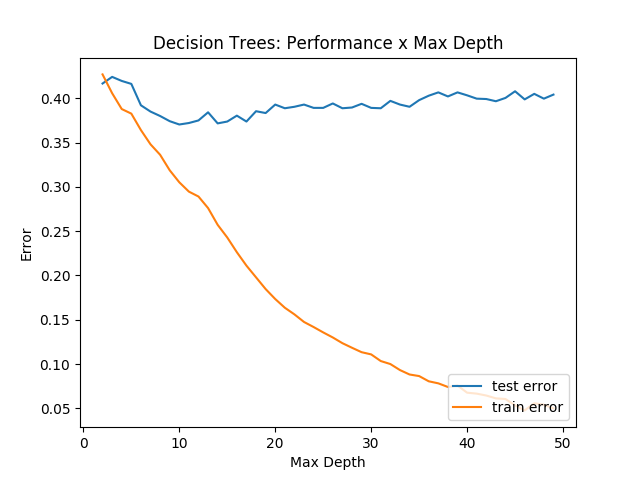
\includegraphics[scale=0.525]{DTMD.png}
% Then, running the algorithm with bag size 2500 and $\texttt{max depth}$ 10:
% \begin{center}
%     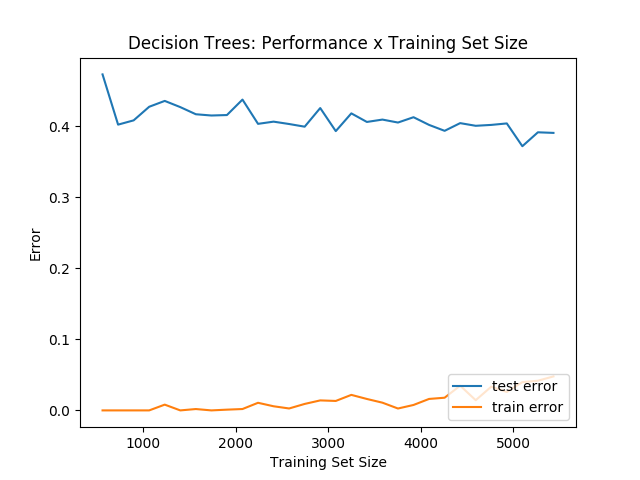
\includegraphics[scale=0.525]{DTTSS.png}
% \end{center}
\begin{wrapfigure}{R}{0.5\textwidth}
\centering
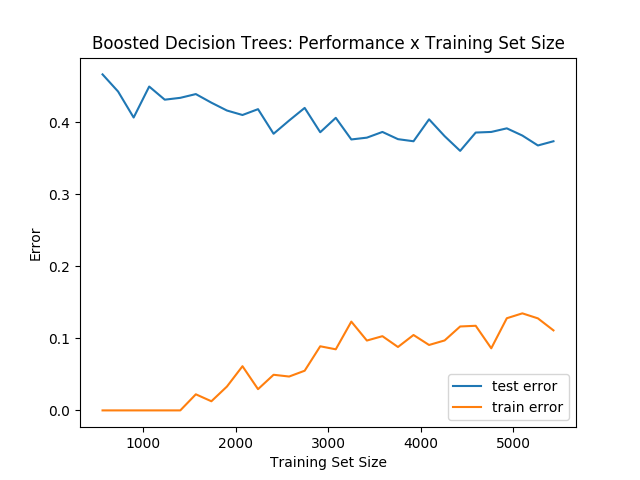
\includegraphics[scale=0.525]{BoostedTSS2.png}
\end{wrapfigure}
Decision trees appear to perform better than the $k$-nearest neighbors technique: the error dips to just below 0.37, the learning curve for test error consistently shrinks, and the learning curve for training error rises slightly from 0. Additionally, it seems that the decision tree requires fewer iterations to reach the same level of error as the $k$-nearest neighbors method of classification. However, despite performing better in accuracy than $k$-nearest neighbors, decision trees are still not a great choice for sentiment analysis; this is due to the fact that words have high complexity (for instance, ``dog'', ``dogs'', and ``doggo'' should be classified under one word class) and the fact that the data has too many important tokens (rather than a few key words, hundreds of thousands of words could be important). My decision tree implements an instance of pruning to prevent the curse of dimensionality; however, a side effect is that several important words could be ignored as partitioning attributes. To lessen the problems caused by high word complexity, I could preprocess my data so that words intended to have the same meaning are identically grouped.
\subsubsection{Boosted Decision Trees}
I chose to boost my decision tree using AdaBoost. In optimizing the bag size for this algorithm, I found that the error remained fairly consistent for bag sizes greater than 2000. I decided to use bag size 4000 in my implementation. Pruning was fulfilled through the use of estimators. With the lowest error, the optimal number of estimators was discovered to be 10. Therefore, I ran the algorithm as a function of training size with bag size 4000 and 10 estimators.
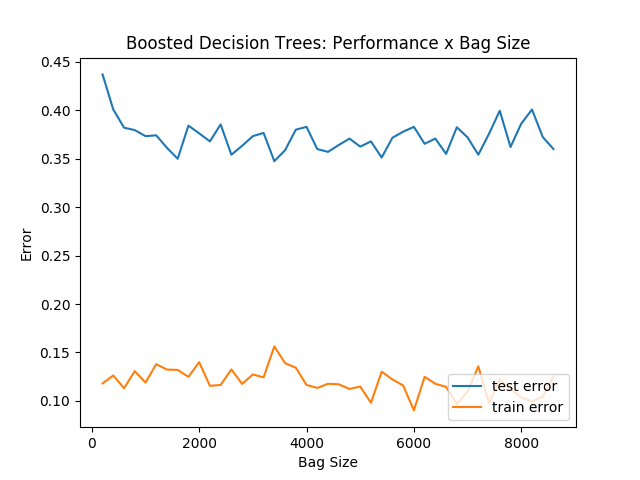
\includegraphics[scale=0.525]{BoostedBS.png}
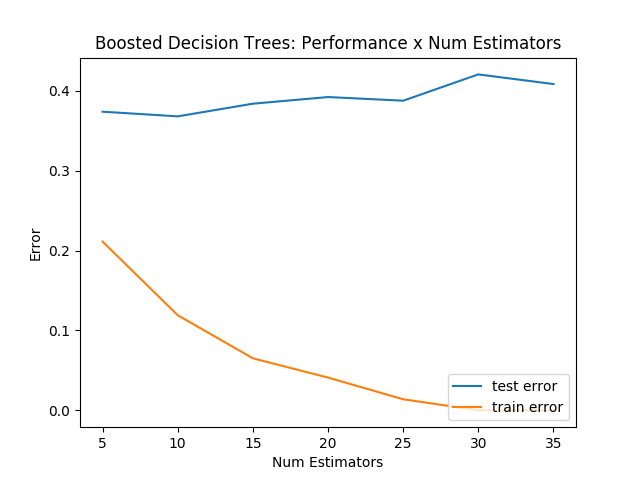
\includegraphics[scale=0.525]{BoostedNE2.png}
% The results are produced below:
% \begin{center}
%     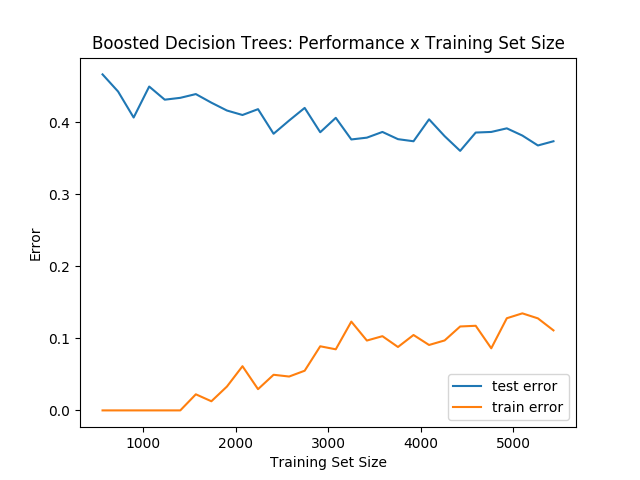
\includegraphics[scale=0.525]{BoostedTSS2.png}
% \end{center}
As expected, the boosted decision tree indeed performed better than the non-boosted decision tree. The two learning curves seem to be converging: the test error steadily diminishes from approximately 0.47 to approximately 0.35, while the training error steadily rises to approximately 0.15. This could be attributed to the fact that normal decision trees do not consider the strength of positive and negative words, whereas a word like ``extraordinary'' contains a stronger positive connotation than a word like ``good''. AdaBoost attempts to remedy this problem by treating each word as a weak classifier. Every time a weak classifier is called, it is given a different distribution over the training examples, thus allowing the algorithm to assign a weight to the classifier. This is particularly beneficial because words such as ``bad'' do not as strongly suggest negative sentiment as words such as ``worst''--a phrase containing the word ``bad'' could still be positive overall! So, the essence of the algorithm itself deems it a more effective one than the standard decision tree.
\subsubsection{Support Vector Machines}
Support vector machines essentially serve to locate the separating hyperplane with the largest margin. In doing this, they can utilize various kernels, which aid in classifying patterns. For this project, I implemented the linear and poly kernels, whose results are reproduced below (linear on the left and poly on the right). It was determined that a bag size of 2000 minimized error for this algorithm. 
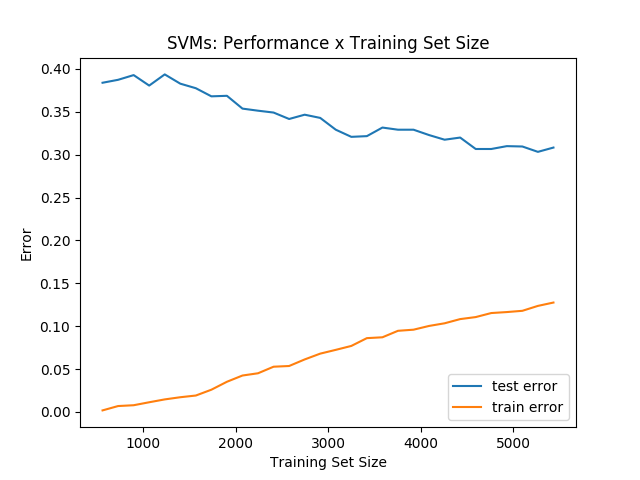
\includegraphics[scale=0.525]{Linear.png}
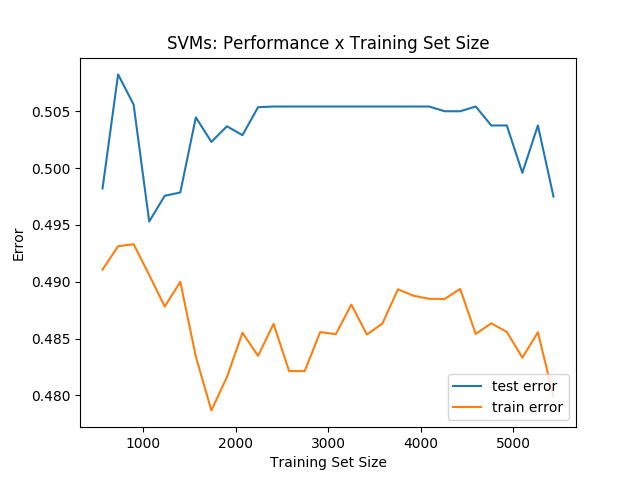
\includegraphics[scale=0.525]{Poly.png}
The support vector machine implementing the linear kernel performed exceedingly well compared to all other algorithms. With an increase in training set size, test error dropped from approximately 0.40 to approximately 0.30, training error grew from approximately 0 to 0.14, and the two learning curves appear to be converging. The linear kernel is probably super effective for this particular dataset since sentiment analysis involves linearly separable text--after all, it is a binary classification problem. Moreover, as previously discussed, sentiment analysis involves numerous important key features; thus, projecting the data onto a multidimensional space wouldn't have much of an effect on performance. Interestingly enough, I also noticed that this algorithm ran significantly faster than the others, especially the $k$-nearest neighbors and boosting algorithms.
\newline\newline
Now, let's consider the poly kernel: I discovered that the error-minimizing degree for the poly kernel is degree 2. However, in spite of this optimization, the error is abnormally high in both the test and training sets, ranging between just below 0.48 and just above 0.50; indeed, the support vector machine implementing the poly kernel actually performed worse than randomly guessing! The trade-off between a more flexible decision boundary and the time and resources required to make it happen was definitely not worth it. By the nature of our linearly separable data, there is no need to map features to such high dimensions. It's notable that unlike its linear counterpart, the poly kernel ran just as slowly as the other algorithms. This is probably also due to the excessive resources required to map so many features to higher dimensions, a process which involves several computationally intensive operations.

\subsubsection{Neural Networks}
Bag size 1500 minimized error in my neural network implementation.  Additionally, I tested various shapes to determine the one that would minimize error. These values were used when running the neural net on varying training set sizes.
\newline\newline
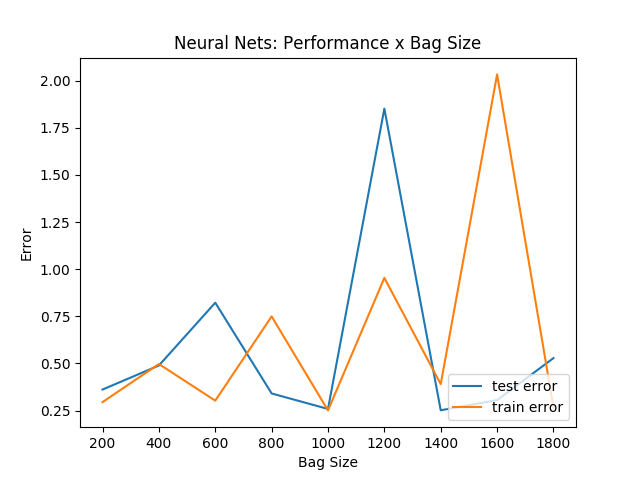
\includegraphics[scale=0.525]{Bag_Size.png}
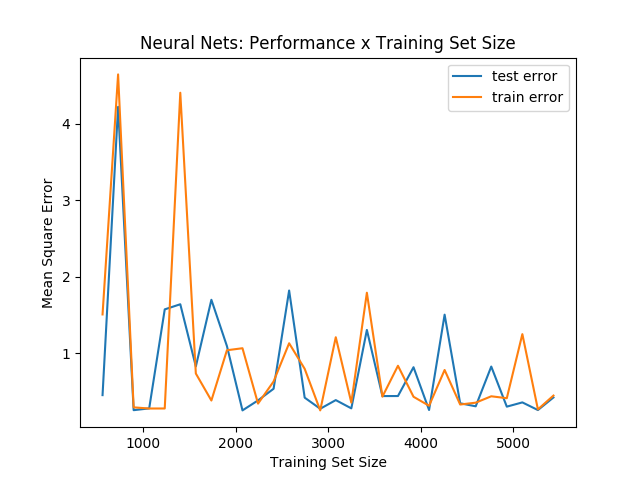
\includegraphics[scale=0.525]{NN_TSS2.png}
I obtained an unusual trend when analyzing error as a function of training set size. Notice that the $y$-axis here is no longer out of 1--while all error graphs for this dataset were calculated using mean squared error ($\texttt{Note:}$ Since this is a binary classification problem with labels and vector values 0 and 1, mean squared error is equal to error percentage.), the neural net implementation compares binary and continuous targets. Analyzing the error with respect to bag size up to 2000 (for the sake of time) reveals that the high complexity of the words is once again a cause for concern--the neural net is not able to distinguish words that actually indicate sentiment and trivial words.
\subsection{Analysis}
Overall, none of the algorithms really did any better than a 35-40\% error rate, or an accuracy rate of 60-65\%. I hypothesize that in addition to the explanations listed above, this may be because some words might take on different values depending on the dataset: for instance, consistency is likely a positive aspect in product reviews but considered a negative aspect in movie reviews (who likes a predictable film?). Therefore, it would take on different sentiment values in the Amazon and IMDb datasets. For future consideration,  many of the problems encountered in this analysis could be minimized through better preprocessing techniques, especially in minimizing the repercussions of using a dataset with many complex features.
\newline\newline
Of the five algorithms, support vector machines implementing linear kernels performed the best, and neural networks performed the worst. With the exception of the basic decision trees and support vector machines implementing linear kernels, all algorithms took numerous hours to run. I'd estimate that $k$-nearest neighbors, boosted decision trees, support vector machines implementing poly kernels, and neural networks took on average four or five hours to run. Basic decision trees and support vector machines implementing linear kernels took just under an hour to run. Cross validation wasn't implemented sheerly due to time constraints, but I believe that it would help in feature selection, which, for the purposes of this analysis, was accomplished by observing error rate while holding all other features constant. This technique was implemented to find the optimal $k$ in $k$-nearest neighbors, the optimal $\texttt{max depth}$ in decision trees, the optimal number of estimators in AdaBoost, the optimal kernel in support vector machines, and the optimal neural network shape and number of hidden layers in neural networks. Select graphs are presented in this analysis; unfortunately, due to the page limit and inefficiencies in $\LaTeX$ formatting, I've decided not to include all graphs.


%---------------------------------------------------------------------------------
% Theory
%---------------------------------------------------------------------------------

\section{Phishing Websites}
% \begin{wrapfigure}{R}{0.5\textwidth}
% \centering
% \includegraphics[scale=0.525]{kNN_CM.png}
% \end{wrapfigure}
\subsection{Algorithms}
The original formatting of the data mandates preprocessing be done before running any algorithms. Edits include breaking trinary classification problems into binary ones using one-hot encoding, and using a 0 and 1 labeling system rather than the original -1 and 1, or -1, 0, and 1 labeling system.
\subsubsection{$K$-Nearest Neighbors}
Like with the sentiment analysis problem, I experimented with the number of neighbors that would maximize accuracy. The accuracy appears to decrease with the addition of more neighbors; I decided to use $k=20$ neighbors for the remaining iterations because the error seems to taper off and stabilize afterwards, and I wanted to strike a balance so that my algorithm neither overfits nor underfits data.
\newline\newline
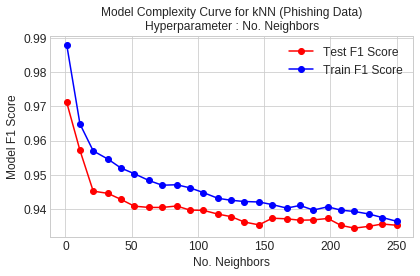
\includegraphics[scale=0.55]{kNN_Model_Complexity.png}
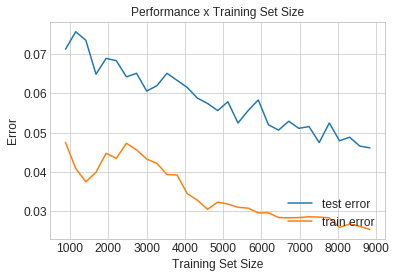
\includegraphics[scale=0.55]{kNN_LC.png}
\newline\newline
Curiously, the test and train errors seem to decrement in a parallel fashion. The test error reaches a low of approximately 0.049, and the training error reaches a low of approximately 0.025. I suspect that this may be caused by overfitting (high variance) in the data. Altering the $k$ value did not seem to affect the learning curves much, but perhaps adding more hyperparameters, such as distance, could remedy this issue. $k$-nearest neighbors runs in about twenty minutes. It has precision value 0.95 and recall value 0.97.

\subsubsection{Decision Trees}
Experimenting with the max tree depth shows that the accuracy stays pretty much consistent after $\texttt{max depth}$ $=15$. Per hyperparameter tuning, the optimal $\texttt{max depth}$ was 8. Furthermore, additional pruning was achieved through hyperparameter analysis on $\texttt{min samples leaf}$, which is a lower bound on the number of samples per leaf that helps decide whether to continue splitting a node or keep the node as a tree leaf. 44 was found to be the optimal value of $\texttt{min samples leaf}$.
\newline\newline
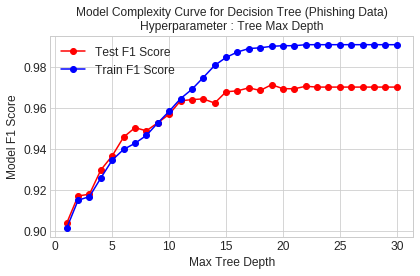
\includegraphics[scale=0.55]{DT_Model_Complexity_1.png}
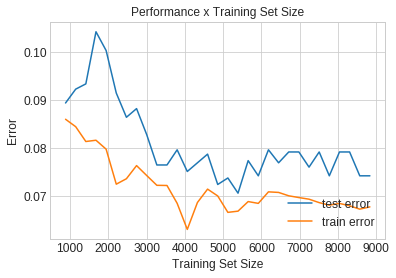
\includegraphics[scale=0.55]{DT_LC.png}
\newline\newline
With a test error low of approximately 0.07 and a training error low of approximately 0.06, the decision tree performed worse than the $k$-nearest neighbors algorithm. This might be in part a consequence of overfitting; although I implemented multiple pruning techniques, the results and learning curves indicate hints of overfitting anyway. To weaken the effect of this problem, I could implement post-pruning techniques, like the error estimation method or the $\chi^2$ test. Regardless, the decision tree ran quickly, terminating in under five minutes. It produced precision value 0.94 and recall value 0.94.

\subsubsection{Boosted Decision Trees}
For this implementation, I used the Gradient boosting algorithm. In tuning hyperparameters, I found that the optimal number of n-estimators was 100, even though the error appeared to stabilize after 50 n-estimators. To prune, I ran another analysis on $\texttt{max depth}$, $\texttt{min samples leaf}$, and a new hyperparameter, learning rate, which shrinks the contribution of each estimator by the respective percentage. It was determined that the optimal $\texttt{max depth}$ is 3, $\texttt{min samples leaf}$ is 44, and learning rate is 0.1 (anything greater resulted in overfitting).
% With these hyperparameters, I iterated over the training set size with the boosted decision tree.
% \begin{wrapfigure}{L}{0.5\textwidth}
% \centering
% \includegraphics[scale=0.55]{Boosted_Modeling_Complexity.png}
% \end{wrapfigure}
\newline
% \includegraphics[scale=0.55]{Boosted_Modeling_Complexity.png}
% \newline\newline
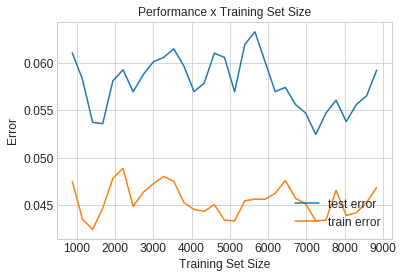
\includegraphics[scale=0.55]{Boosted_LC.png}
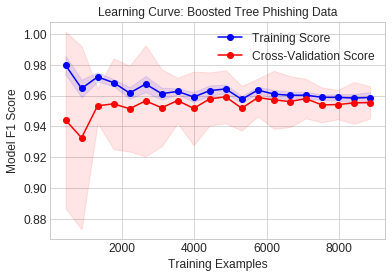
\includegraphics[scale=0.55]{Boosted_Learning_Curve.png}
\newline\newline
Boosted decision trees performed slightly better than their non-boosted counterparts, with the test error dropping to as low as approximately 0.053 and the training error dropping to as low as approximately 0.043. Moreover, examine the cross-validation graph. Notice that when the training set size is small, training accuracy is high but cross-validation score is low because of overfitting. As the number of training examples increases, the model doesn't overfit as easily; therefore, the training score slightly decreases, but the cross-validation scores trends upwards because the model is better suited to account for new data. Like the standard decision tree, the boosted decision tree ran fairly quickly, and too terminated in under five minutes. It had precision value 0.94 and recall value 0.97.
\subsubsection{Support Vector Machines}
For the phishing websites dataset, I implemented the linear, poly (with $2\leq \deg\leq 8$), radial basis function, and sigmoid kernels for support vector machines. Notice that past degree 5, the poly kernel's accuracy drops significantly. It appears that the default radial basis function kernel had the highest accuracy, so it was the kernel used for the rest of the algorithms' iterations. The trade-off, however, for the higher accuracy of the radial basis function kernel is its runtime. The rgb kernel took five seconds longer to terminate than other kernels, all of which terminated almost instantaneously. 
\newline\newline
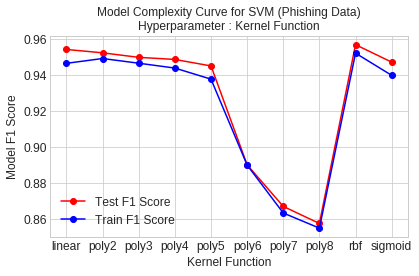
\includegraphics[scale=0.55]{SVM_Model_Complexity_2.png}
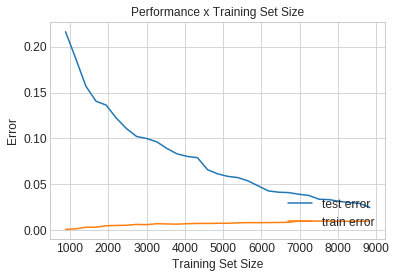
\includegraphics[scale=0.55]{SVM_LC.png}
\newline\newline
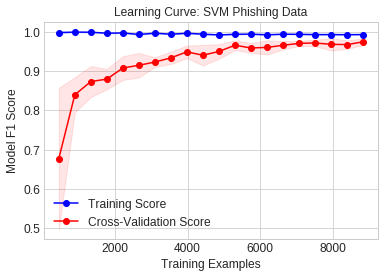
\includegraphics[scale=0.55]{SVM_Learning_Curve_2.png}
\quad\quad\quad\quad
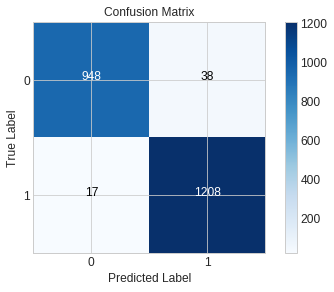
\includegraphics[scale=0.55]{SVM_Confusion_Matrix_2.png}
\newline\newline
The support vector machine with rgb kernel was super effective: the test and train error converge at approximately 0.015. This fact is reflected in the cross-validation curve as well: the training score and cross-validation score converge near an accuracy of 1! The high accuracy can be attributed to the support vector machine's regularization parameter that removes the burden of overfitting if the ideal kernel is selected. It cannot be guaranteed that support vector machines with other kernels will produce errors as low as the rgb kernel's. The support vector machine with rgb kernel has precision 0.97 and recall 0.99.
\subsubsection{Neural Networks}
Testing was conducted to determine the optimal hyperparameters for this algorithm. Per hyperparameter tuning, I found the optimal initial learning rate to be 0.01 and the optimal size of the hidden layers to be 100. It's important to note that the neural net trained for an excessively long period of time, especially compared to the other algorithms.
\newline\newline
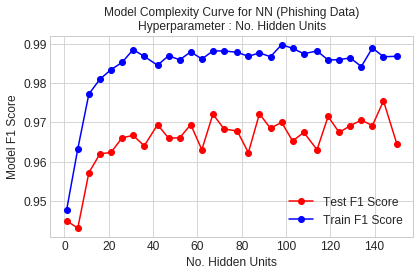
\includegraphics[scale=0.55]{NN_Model_Complexity_Curve.png}
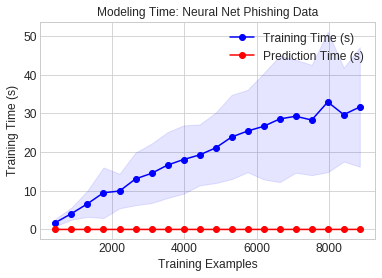
\includegraphics[scale=0.55]{NN_Modeling_Time.png}
\newline\newline
Although the error plot for this the training set spikes when the training set is small, the test error learning curve experiences a relatively consistent downward trend. Upon further examination of the cross-validation score, notice that while the cross-validation score is on the rise, the training score remains relatively stable. The downward trend of the test error learning curve suggests that should it be given more data to train our algorithm on, the neural network could produce an error similar to that of support vector machines. This iteration, it resulted in a precision rate of 0.98 and recall rate of 0.97.
\newline\newline
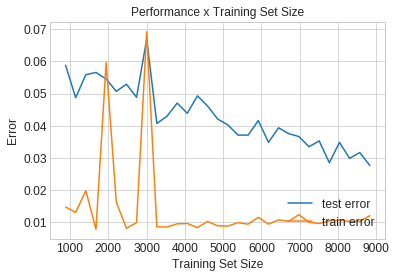
\includegraphics[scale=0.55]{NN_LC.png}
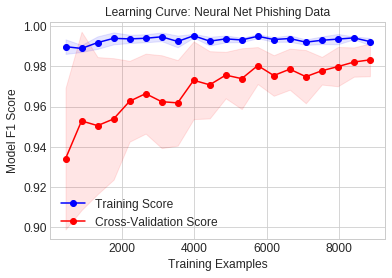
\includegraphics[scale=0.55]{NN_Learning_Curve.png}
\subsection{Analysis}
\begin{wrapfigure}{L}{0.5\textwidth}
\centering
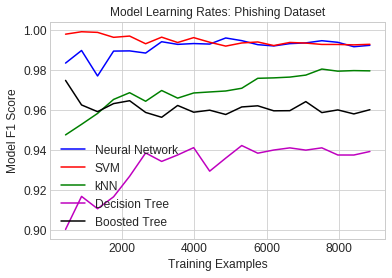
\includegraphics[scale=0.525]{MLR.png}
\end{wrapfigure}
The five supervised learning algorithms performed relatively well on the phishing email dataset, especially compared to the performance on the sentiment analysis dataset. On average, the algorithms' error was a mere 0.028. This is probably due to the fact that the phishing email dataset has more clearly defined labels and not-too-many features, aspects not present in the sentiment analysis dataset. For future consideration, more work could be done on tuning hyperparameters to avoid overfitting, a problem I encountered in the $k$-nearest neighbors and decision tree implementations. Cross validation was implemented to discover trends in overfitting data, although I'll admit I could've been better about fixing that issue. Parameters were tuned to optimize the algorithm, most of which are shown.
\newline
% 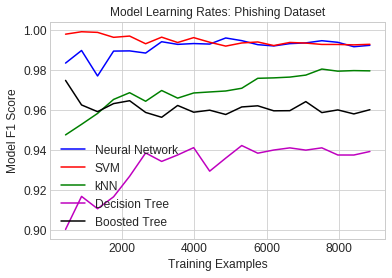
\includegraphics[scale=0.55]{MLR.png}
\newline
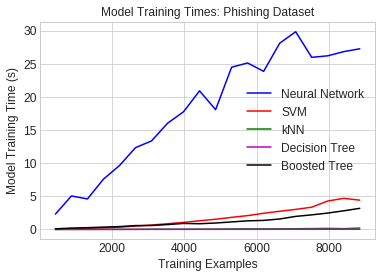
\includegraphics[scale=0.55]{Time_Comparison.png}
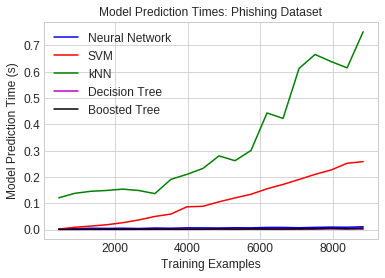
\includegraphics[scale=0.55]{TIme_Predict.png}
\newline
The best algorithm for the phishing websites dataset is the support vector machine with rgb; it achieved the lowest error and didn't take ridiculously long to run. It can be inferred from these graphs that neural networks are the most training-time-expensive algorithm, while $k$-nearest neighbors is the most prediction-time-expensive algorithm. The suboptimal speed of my neural network is expected given that I used a multilayer perceptron, a type of deep neural network. Programming and debugging my neural network had to be the most time-intensive task of the five, solely because some errors weren't apparent to me until hours into training. On the other hand, $k$-nearest neighbor's lag can be attributed to lazy training. In other words, $k$-nearest neighbors collects and retains all training data for the duration of the program. Each of the other algorithms simply discards the data after training completion--this definitely would contribute to $k$-nearest neighbor's sluggish performance.

% If you want to add mathematical equations, this may be done either this way: $a +  b \neq \frac{a}{b}$. You may also add Greek letters like this: $\alpha$.\\ 

% \blindtext % Some blind text

% % Including figures
% \begin{figure}[htpb!] % Defines figure environment
%     \centering % Centers your figure
% \includegraphics[scale=0.8]{figure/figure.png} % Includes your figure and defines the size
%     \caption{A circle} % For your caption
%     \label{fig:my_label} % If you want to label your figure for in-text references
% \end{figure}

% \blindtext % Some blind text

% % Including tables
% %   Simple table
% \begin{table}[] % Add htpb! to make sure that table is where it should be
%     \centering
%     \begin{tabular}{c|c}
%         Saturday & Sunday \\
%         12 & 18
%     \end{tabular}
%     \caption{Overview of the weekend}% Caption for tables
%     \label{tab:weekend} % Reference for in-line referencing
% \end{table}

% %   Table with table generator
% \begin{table}[] % Add htpb! to make sure that table is where it should be
%     \centering
% \begin{tabular}{@{}lll@{}}
% \toprule
%   & A   & B \\ \midrule
% C & 100 & 2 \\
% D & 3   & 5 \\ \bottomrule
% \end{tabular}
%     \caption{Random numbers} % Caption for tables
%     \label{tab:numbers} % Reference for in-line referencing
% \end{table}

% %----------------------------------------------------------------------------------------
% % Research design
% %----------------------------------------------------------------------------------------

% \section{Research Design}

% \blindtext % Some blind text

%----------------------------------------------------------------------------------------
% Analysis
%----------------------------------------------------------------------------------------

\section{Analysis and Conclusion}
In completing this homework assignment, not only did I come to learn and understand the workings behind $k$-nearest neighbors, decision trees, boosting, support vector machines, and neural networks, but also I was able to experiment with their hyperparameters, various techniques used to prevent and reduce overfitting, and work with (pre)processing enormous quantities of data. I enjoyed my datasets, even though at times, they could be difficult to work with. And although I didn't obtain the best results, the errors and accuracies presented in this paper were the result of many hours of optimization.
% \blindtext % Some blind text

% %----------------------------------------------------------------------------------------
% % Conclusion
% %----------------------------------------------------------------------------------------

% \section{Conclusion}

% \blindtext % Some blind text

% %----------------------------------------------------------------------------------------
% % Bibliography
% %----------------------------------------------------------------------------------------
% \newpage % Includes a new page

% \pagenumbering{roman} % Changes page numbering to roman page numbers
% %\bibliography{literature}

% \bibliography{literature.bib} % Add the filename of your bibliography
% \bibliographystyle{apsr} % Defines your bibliography style

% % For citing, please see this sheet: http://merkel.texture.rocks/Latex/natbib.php

% %----------------------------------------------------------------------------------------
% % Appendix
% %----------------------------------------------------------------------------------------
% \newpage % Includes a new page
% \section*{Appendix} % Stars disable section numbers
% % \appendix % Uncomment if you want to add an "automatic" appendix
% \pagenumbering{Roman} % Changes page numbering to Roman page numbers

% \blindtext % Adds some blind text

% %----------------------------------------------------------------------------------------
% % Declaration
% %----------------------------------------------------------------------------------------
% \newpage % Includes a page break
% \thispagestyle{empty} % Leaves the page style empty (no page number, no header, no footer)
% \section*{Statutory Declaration} % Stars disable section numbers

% \begin{otherlanguage}{german}
% Hiermit versichere ich, dass diese Arbeit von mir pers\"{o}nlich verfasst ist und dass ich keinerlei fremde Hilfe in Anspruch genommen habe. Ebenso versichere ich, dass diese Arbeit oder Teile daraus weder von mir selbst noch von anderen als Leistungsnachweise andernorts eingereicht wurden. W\"{o}rtliche oder sinngem\"{a}{\ss}e \"{U}bernahmen aus anderen Schriften und Ver\"{o}ffentlichungen in gedruckter oder elektronischer Form sind gekennzeichnet. S\"{a}mtliche Sekund\"{a}rliteratur und sonstige Quellen sind nachgewiesen und in der Bibliographie aufgef\"{u}hrt. Das Gleiche gilt f\"{u}r graphische Darstellungen und Bilder sowie f\"{u}r alle Internet-Quellen. Ich bin ferner damit einverstanden, dass meine Arbeit zum Zwecke eines Plagiatsabgleichs in elektronischer Form anonymisiert versendet und gespeichert werden kann. Mir ist bekannt, dass von der Korrektur der Arbeit abgesehen und die Pr\"{u}fungsleistung mit nicht ausreichend bewertet werden kann, wenn die Erkl\"{a}rung nicht erteilt wird.
% \end{otherlanguage}

% \vspace*{1in} % Adds extra space between two paragraphs

% \noindent I hereby declare that the paper presented is my own work and that I have not called upon the help of a third party. In addition, I affirm that neither I nor anybody else has submitted this paper or parts of it to obtain credits elsewhere before. I have clearly marked and acknowledged all quotations or references that have been taken from the works of others. All secondary literature and other sources are marked and listed in the bibliography. The same applies to all charts, diagrams and illustrations as well as to all Internet resources. Moreover, I consent to my paper being electronically stored and sent anonymously in order to be checked for plagiarism. I am aware that the paper cannot be evaluated and may be graded ``failed'' (``nicht ausreichend'') if the declaration is not made.\\

% %\vspace*{1in} % Adds extra space

% % Add field for signature, date, and place
% \hfill \signature{} 


%---------------------------------------------------------------------------------

\end{document}
